%%%%%%%%%%%%%%%%%%%%%%%%%%%%%%%%%%%%%%%%%%%%%%%%%%%%%%%%%%%%%%%%%%%%%%%%%%%%%%%%
%
% https://www.sharelatex.com/learn/Beamer
%
%%%%%%%%%% 
\documentclass{beamer}
	\usetheme{ACUAS}
%	\usetheme{Madrid}
%
% 	- Hiding the presentation controls in LaTeX beamer presentation [closed]
%		- https://stackoverflow.com/questions/3017030/hiding-the-presentation-controls-in-latex-beamer-presentation
\setbeamertemplate{navigation symbols}{}


%%%%%%%%%%%%%%%%%%%%%%%%%%%%%%%%%%%%%%%%%%%%%%%%%%%%%%%%%%%%%%%%%%%%%%%%%%%%%%%%
%
% Packages
%
%%%%%%%%%% 
\usepackage{fontspec}
\usepackage{lmodern}
\usepackage{graphicx}
	\graphicspath{{./logos/}{./bilder/}}


%%%%%%%%%%%%%%%%%%%%%%%%%%%%%%%%%%%%%%%%%%%%%%%%%%%%%%%%%%%%%%%%%%%%%%%%%%%%%%%%
%
% Information to be included in the title page
%
%%%%%%%%%%
\title[RO-SLAM mittels UWB]{Range-Only Simultaneous Localization and Mapping mittels Ultra-Wideband}
%\subtitle{}
\author{Albert Kasdorf}
\institute[FH Aachen]
{
	FH Aachen\\
	Fachbereich Elektrotechnik und Informationstechnik\\
	Ingenieur-Informatik
}
\date{2018}


\begin{document}


%%%%%%%%%%%%%%%%%%%%%%%%%%%%%%%%%%%%%%%%%%%%%%%%%%%%%%%%%%%%%%%%%%%%%%%%%%%%%%%%
%
% Titelseite
%
%%%%%%%%%%
\frame{\titlepage}


%%%%%%%%%%%%%%%%%%%%%%%%%%%%%%%%%%%%%%%%%%%%%%%%%%%%%%%%%%%%%%%%%%%%%%%%%%%%%%%%
%
% Inhaltsverzeichnis?
%
%%%%%%%%%%
%\begin{frame}
%\frametitle{Inhaltsverzeichnis}
%\tableofcontents
%\end{frame}


%%%%%%%%%%%%%%%%%%%%%%%%%%%%%%%%%%%%%%%%%%%%%%%%%%%%%%%%%%%%%%%%%%%%%%%%%%%%%%%%
%
% 
%
%%%%%%%%%%
\begin{frame}
	\frametitle{Begrifflichkeiten}
	\begin{itemize}
		\item Lokalisierung (engl. Localization)
		\item Kartenerstellung (engl. Mapping)
		\item SLAM
	\end{itemize}
\end{frame}


%%%%%%%%%%%%%%%%%%%%%%%%%%%%%%%%%%%%%%%%%%%%%%%%%%%%%%%%%%%%%%%%%%%%%%%%%%%%%%%%
%
% 
%
%%%%%%%%%%
\begin{frame}
	\frametitle{Range-Only Simultaneous Localization and Mapping}
	Was ist das Ziel?
	Wie kommt man da hin?
\end{frame}


%%%%%%%%%%%%%%%%%%%%%%%%%%%%%%%%%%%%%%%%%%%%%%%%%%%%%%%%%%%%%%%%%%%%%%%%%%%%%%%%
%
% 
%
%%%%%%%%%%
\begin{frame}
	\frametitle{UWB-Modul}

	\begin{columns}
		\column{0.5\textwidth}
		\begin{itemize}
			\item UWB (Bandbreite)
			\item DecaWave UWB-Modul
			\item Verarbeitungseinheit
			\item Datenaustausch
			\item Ladeelektronik
			\item ...
		\end{itemize}
		
		\column{0.5\textwidth}
			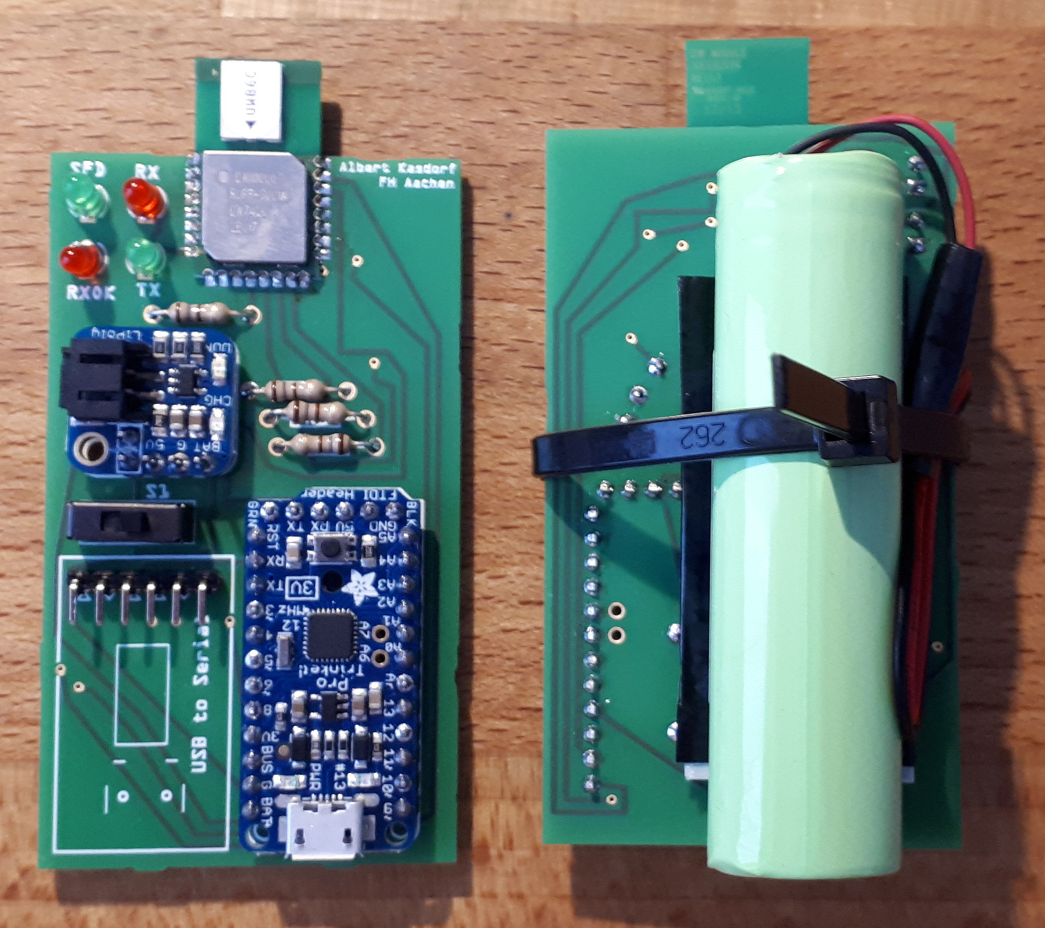
\includegraphics[scale=0.2]{uwb_modul}
			
	\end{columns}
\end{frame}


%%%%%%%%%%%%%%%%%%%%%%%%%%%%%%%%%%%%%%%%%%%%%%%%%%%%%%%%%%%%%%%%%%%%%%%%%%%%%%%%
%
% 
%
%%%%%%%%%%
\begin{frame}
	\frametitle{Kalibierung der Entfernungsmessung (1)}
	\begin{columns}
		\column{0.5\textwidth}
		\begin{itemize}
			\item DecaWave Verfahren
			\begin{itemize}
				\item Genetischer Algorithmus
				\item Instabiles Verfahren
			\end{itemize}
			
			\item LGS
		\end{itemize}
		
		\column{0.5\textwidth}
			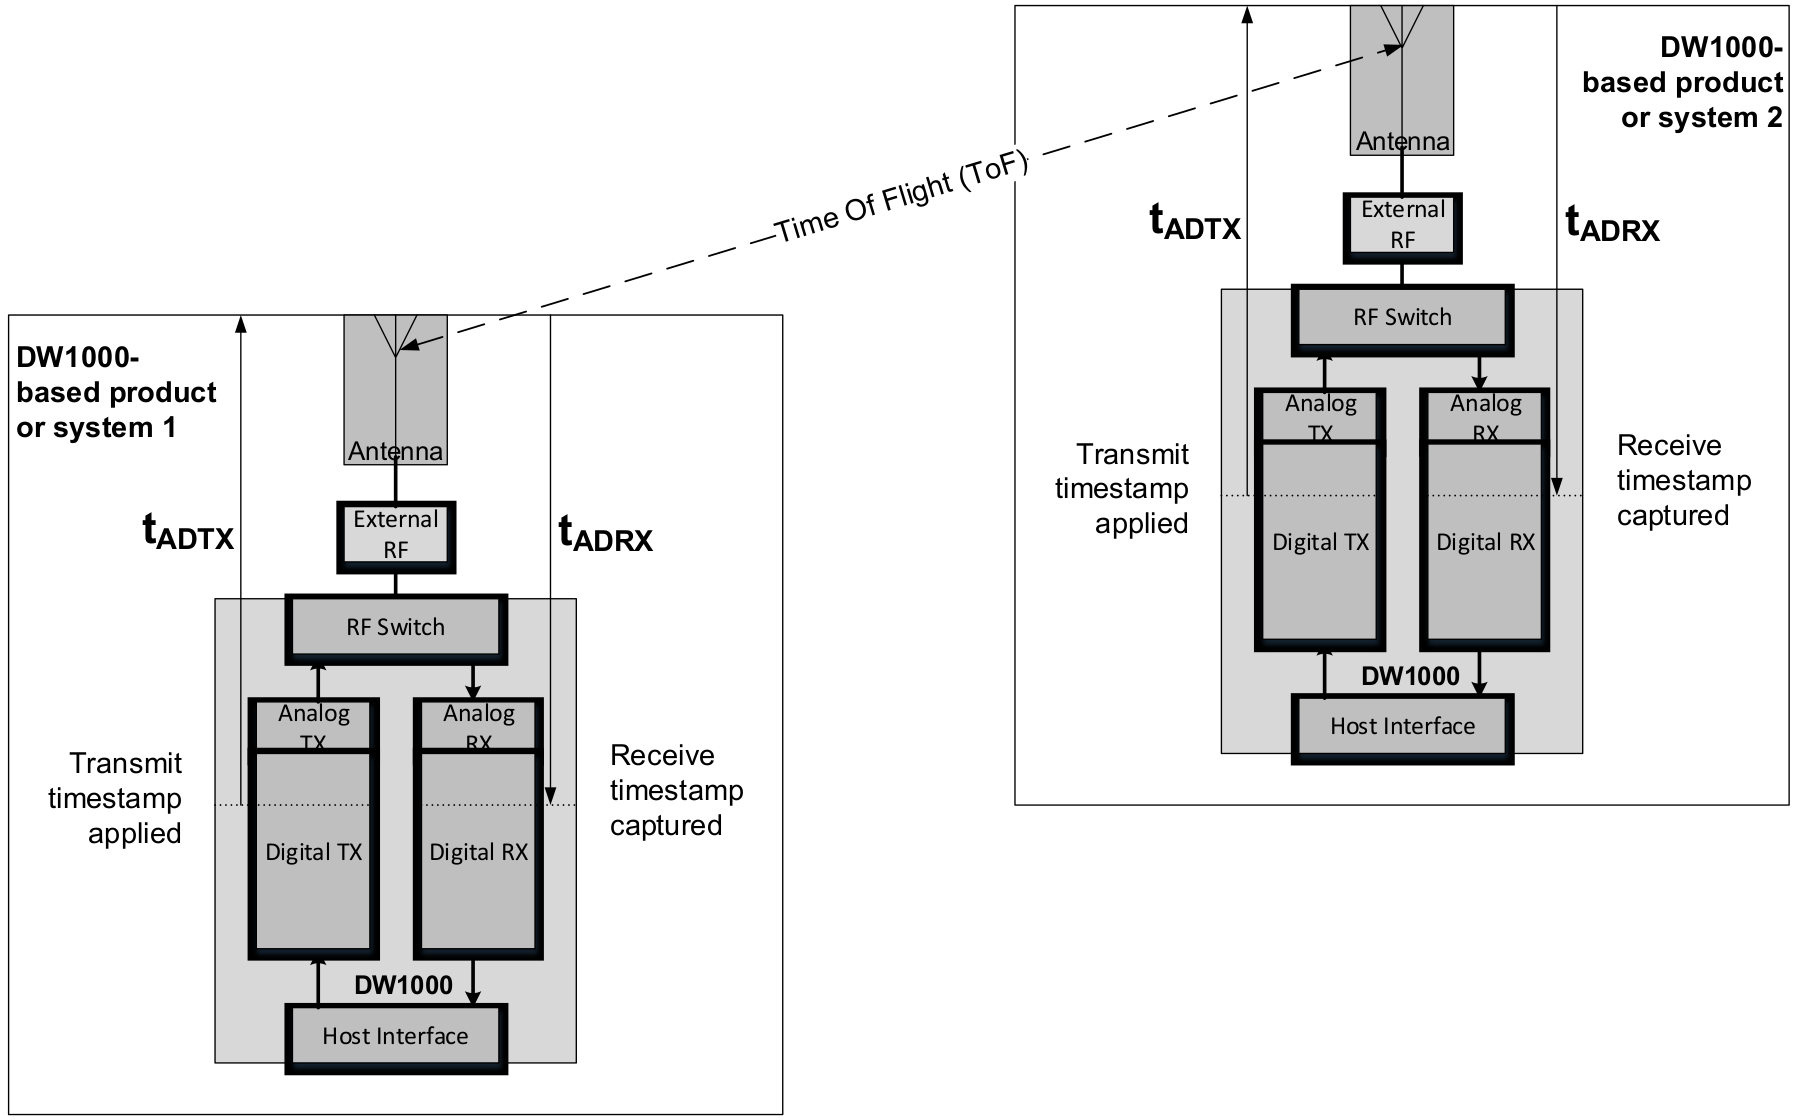
\includegraphics[scale=0.09]{decawave2014calibration_fig1}
	\end{columns}
\end{frame}


%%%%%%%%%%%%%%%%%%%%%%%%%%%%%%%%%%%%%%%%%%%%%%%%%%%%%%%%%%%%%%%%%%%%%%%%%%%%%%%%
%
% 
%
%%%%%%%%%%
\begin{frame}
	\frametitle{Kalibierung der Entfernungsmessung (2)}
	\centering
	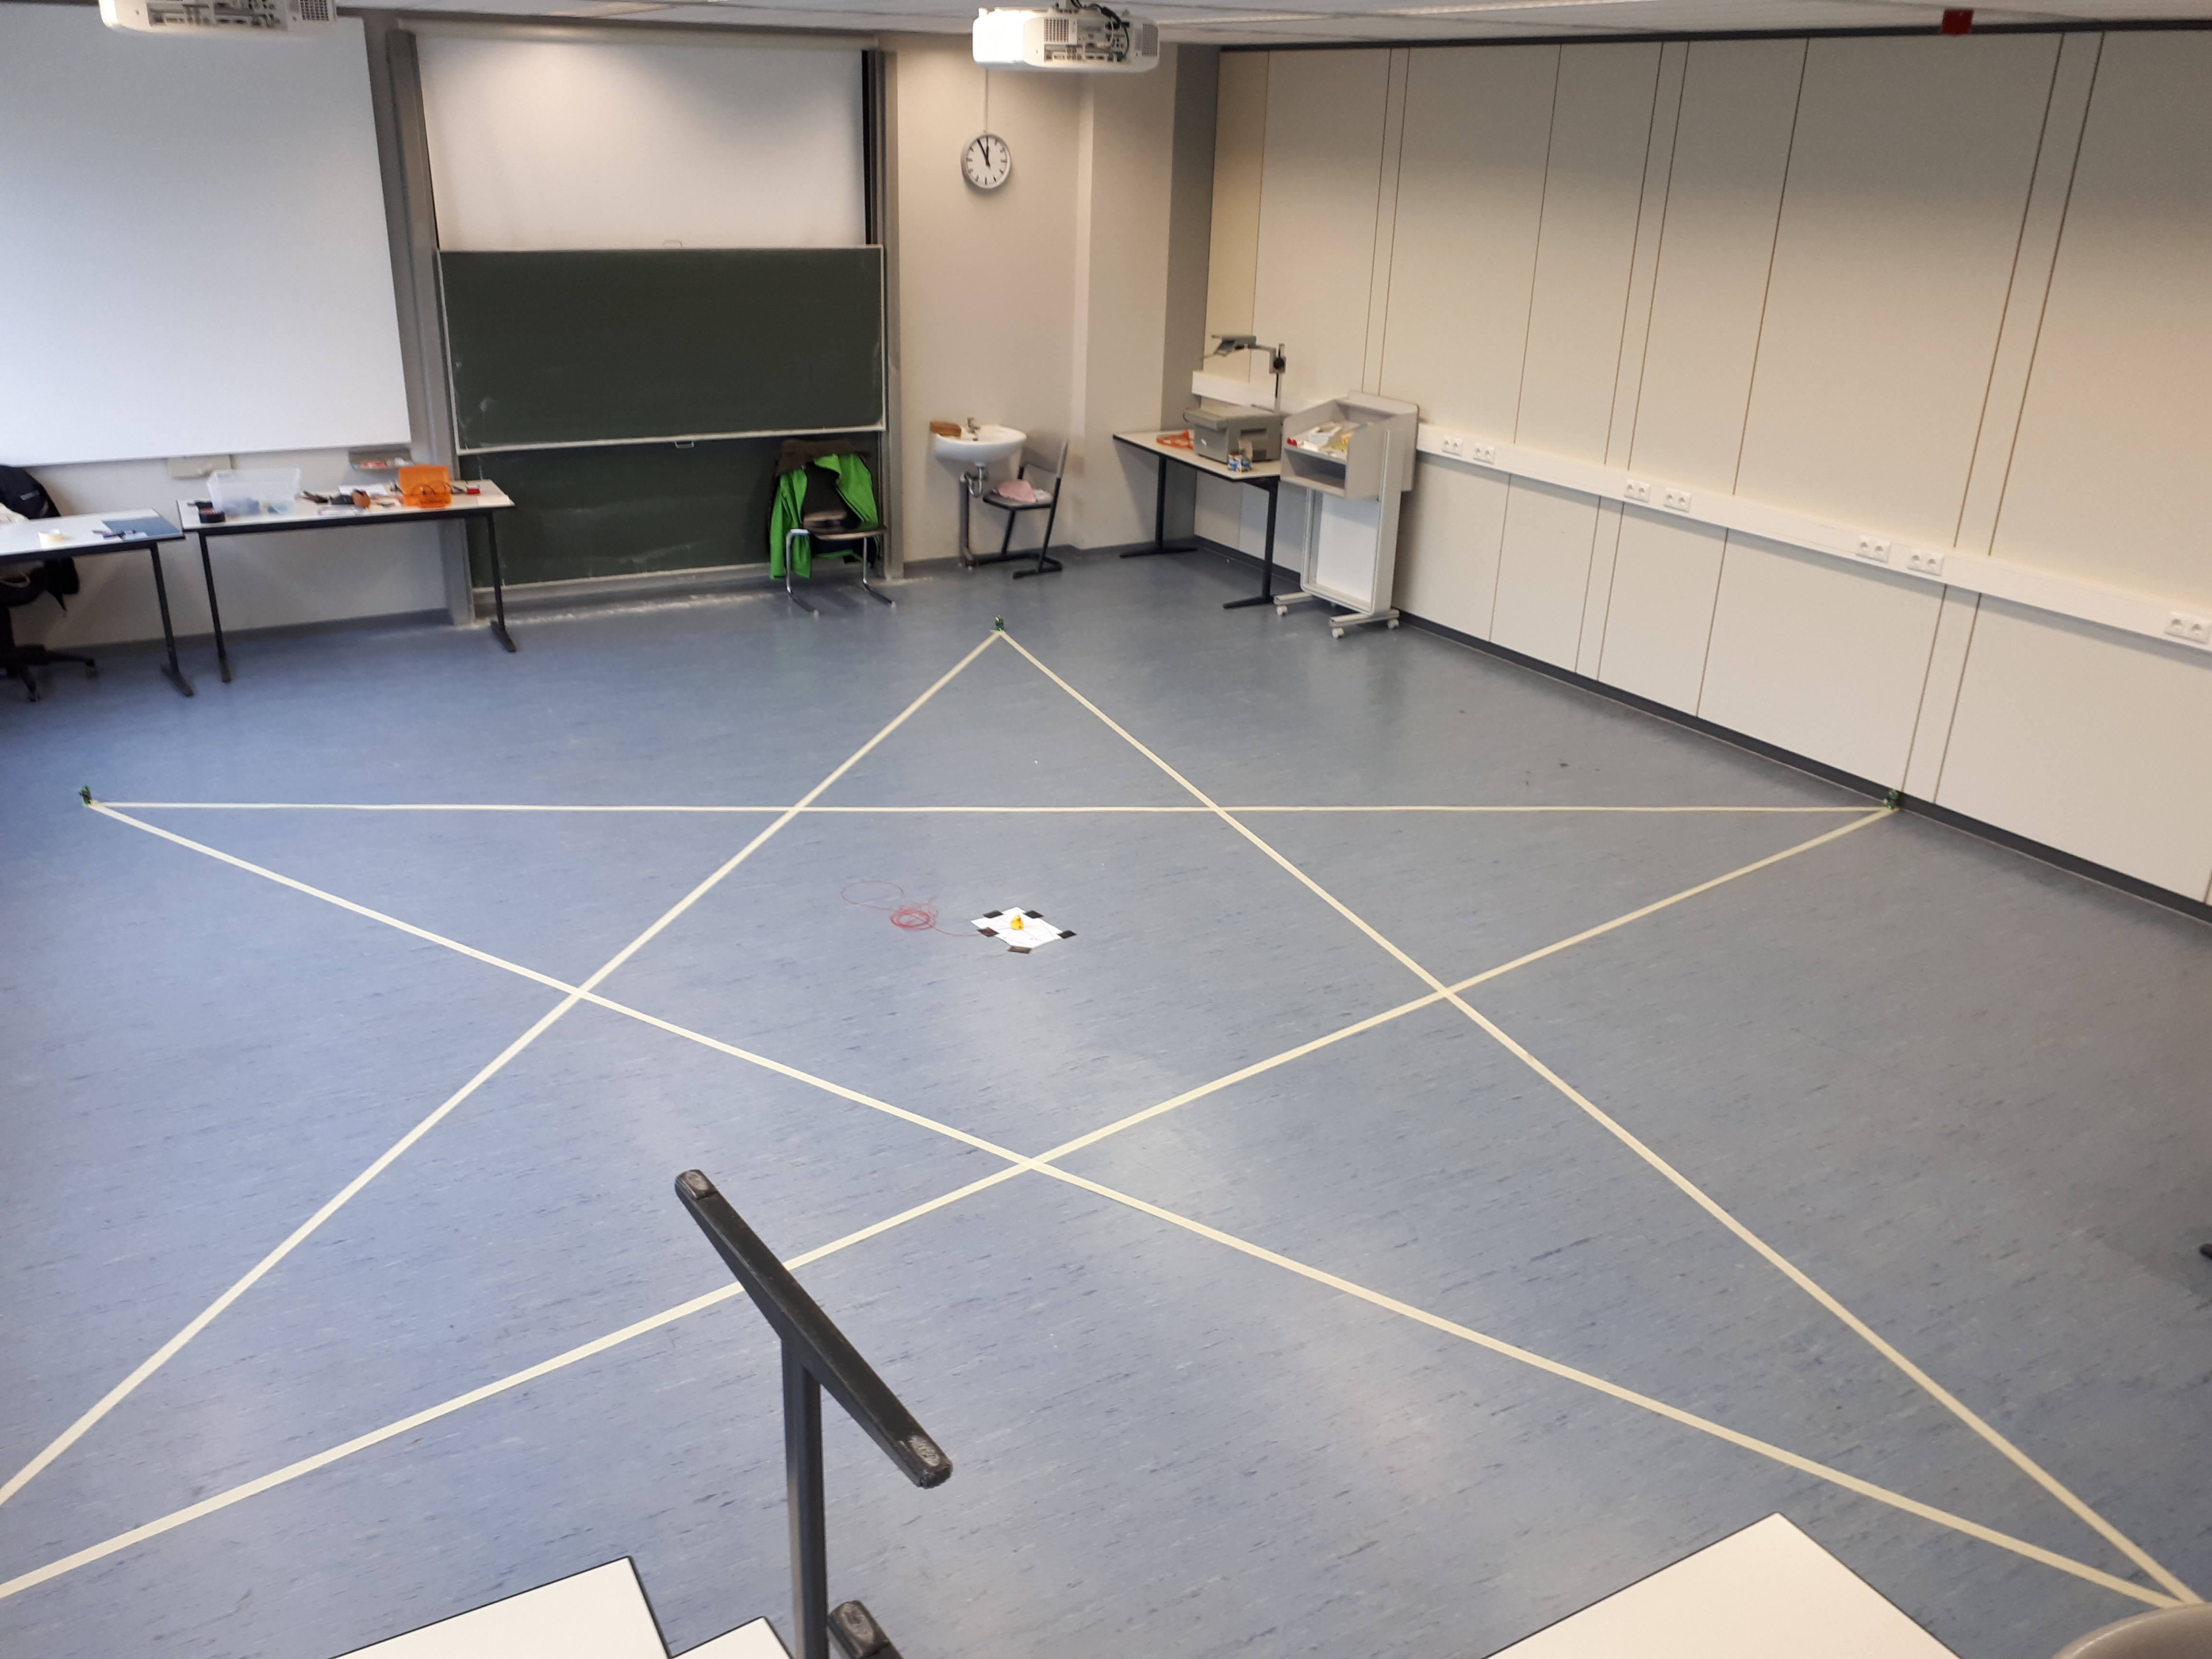
\includegraphics[scale=0.06]{calibration_pentagram}
\end{frame}


%%%%%%%%%%%%%%%%%%%%%%%%%%%%%%%%%%%%%%%%%%%%%%%%%%%%%%%%%%%%%%%%%%%%%%%%%%%%%%%%
%
% 
%
%%%%%%%%%%
\begin{frame}
	\frametitle{Ergebnisse der Entfernungsmessung}
	\begin{columns}
		\column{0.5\linewidth}
			\centering
			
			LOS
			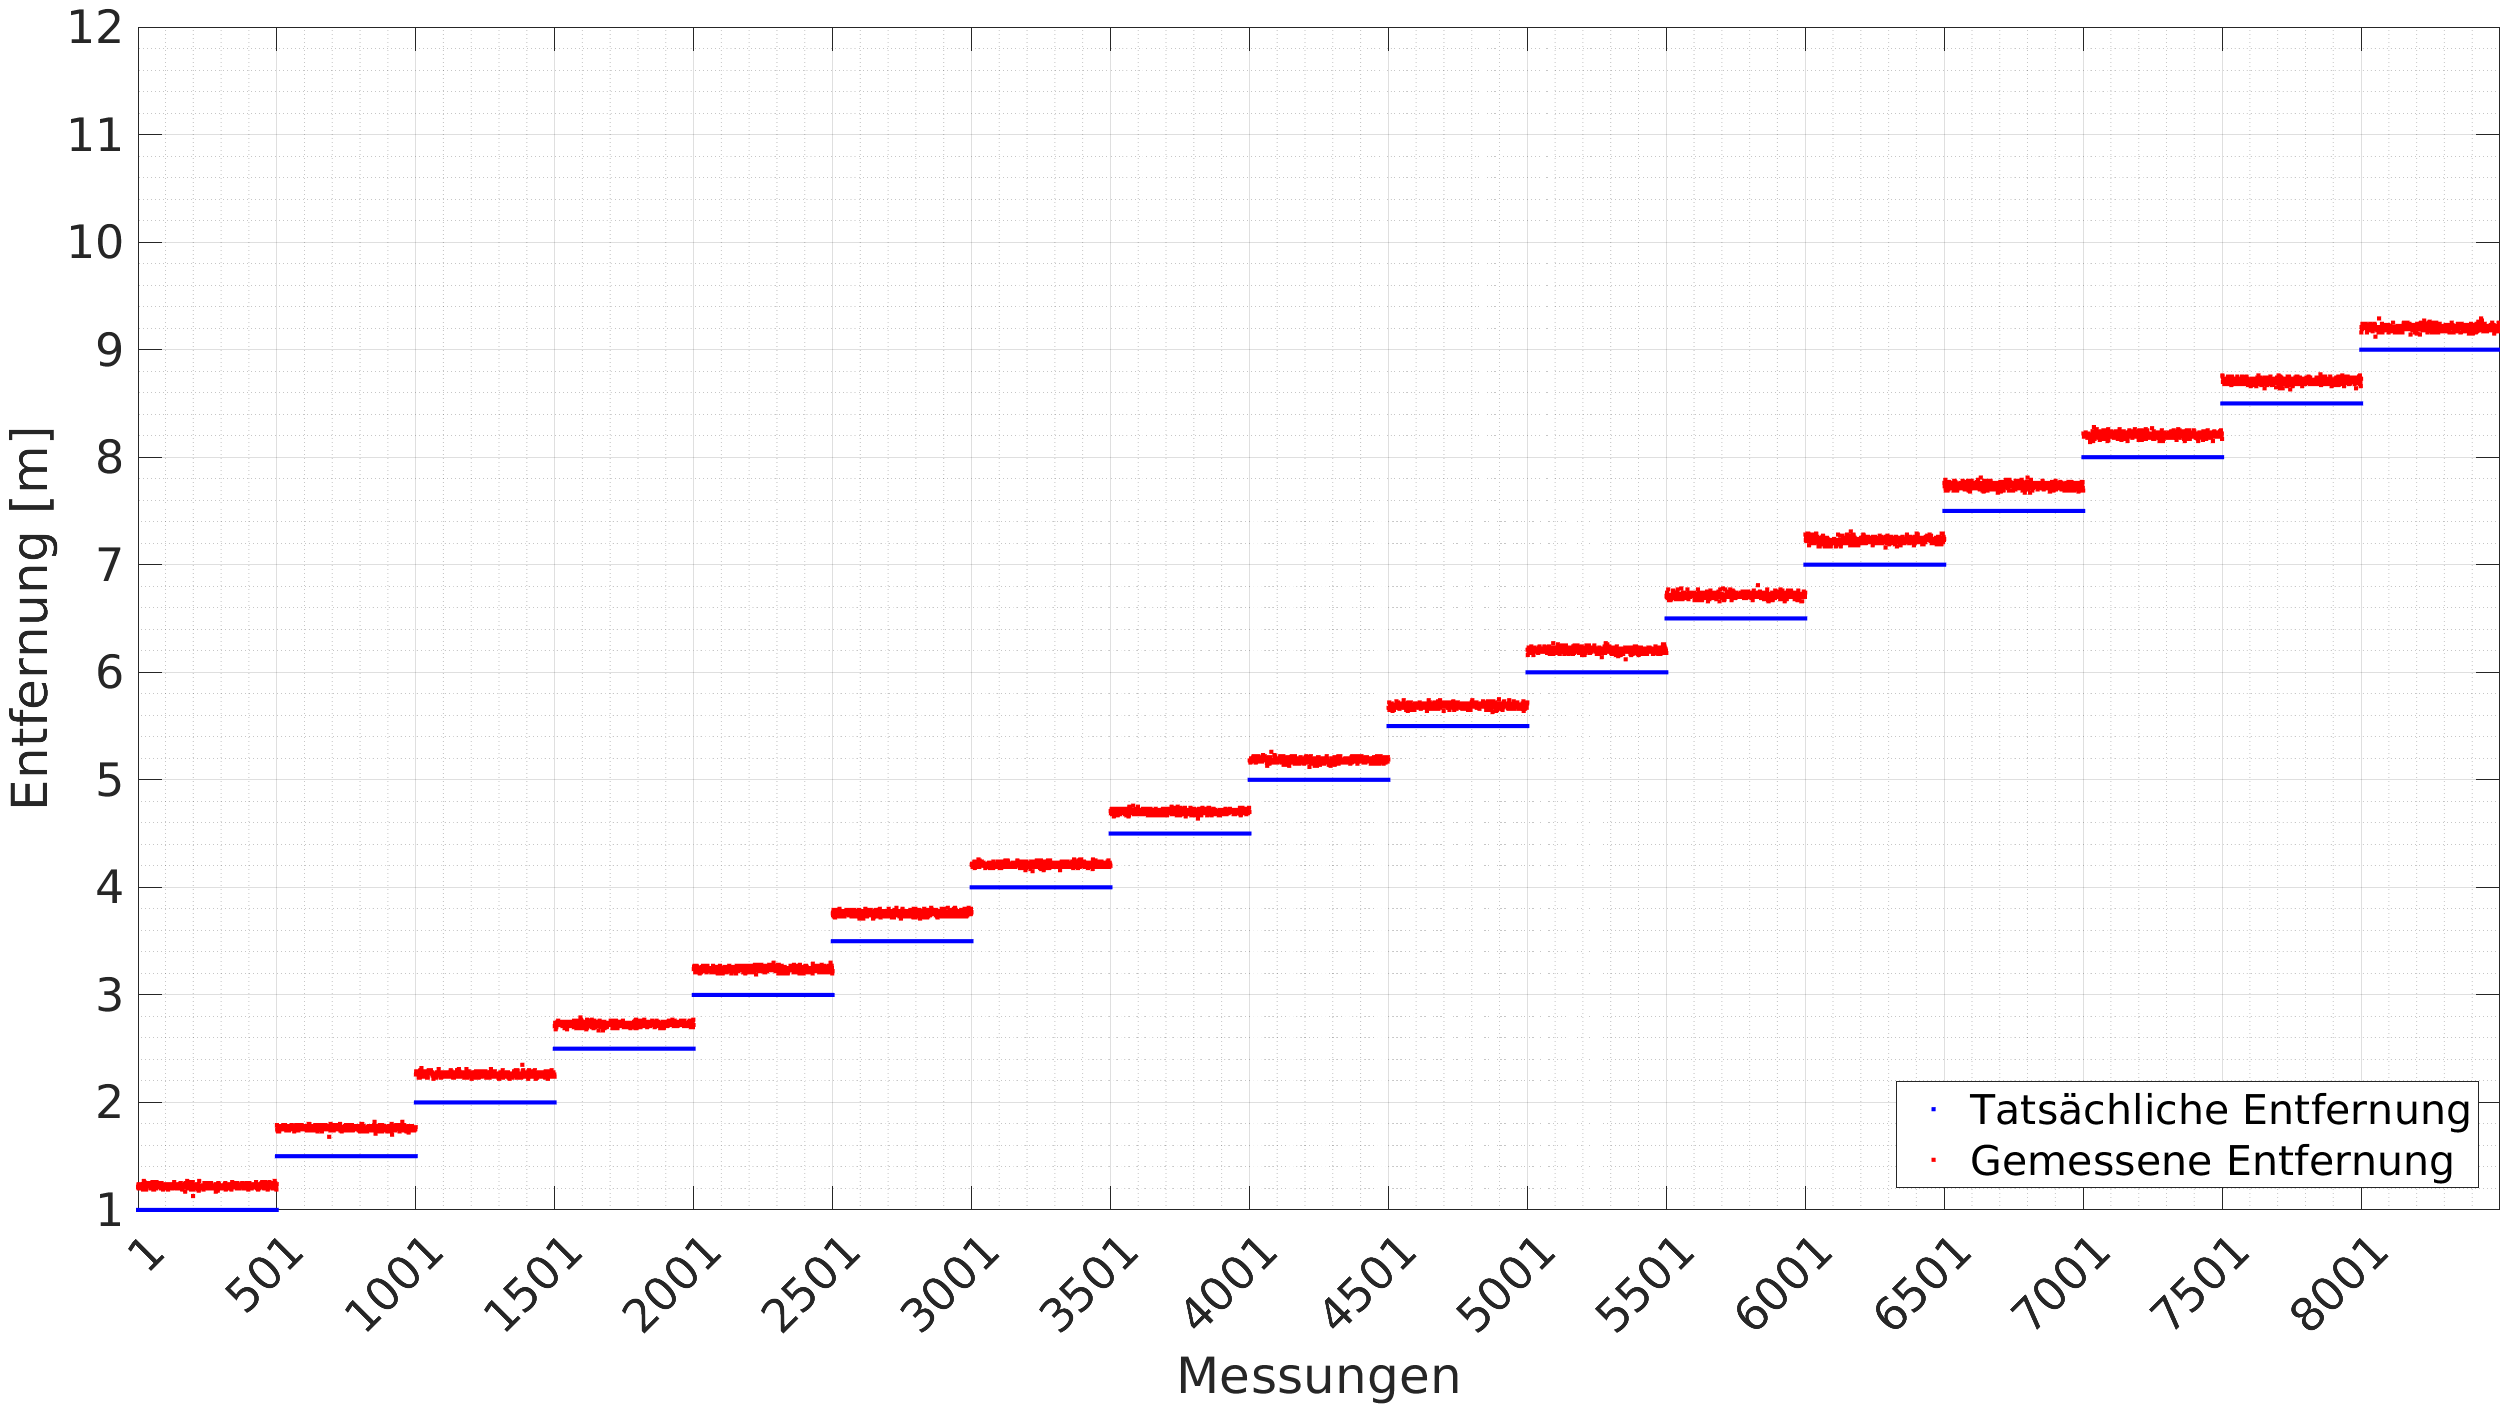
\includegraphics[scale=0.14]{entfernungsmessung_2018_01_20_los}
			
			NLOS mit Metall (1)
			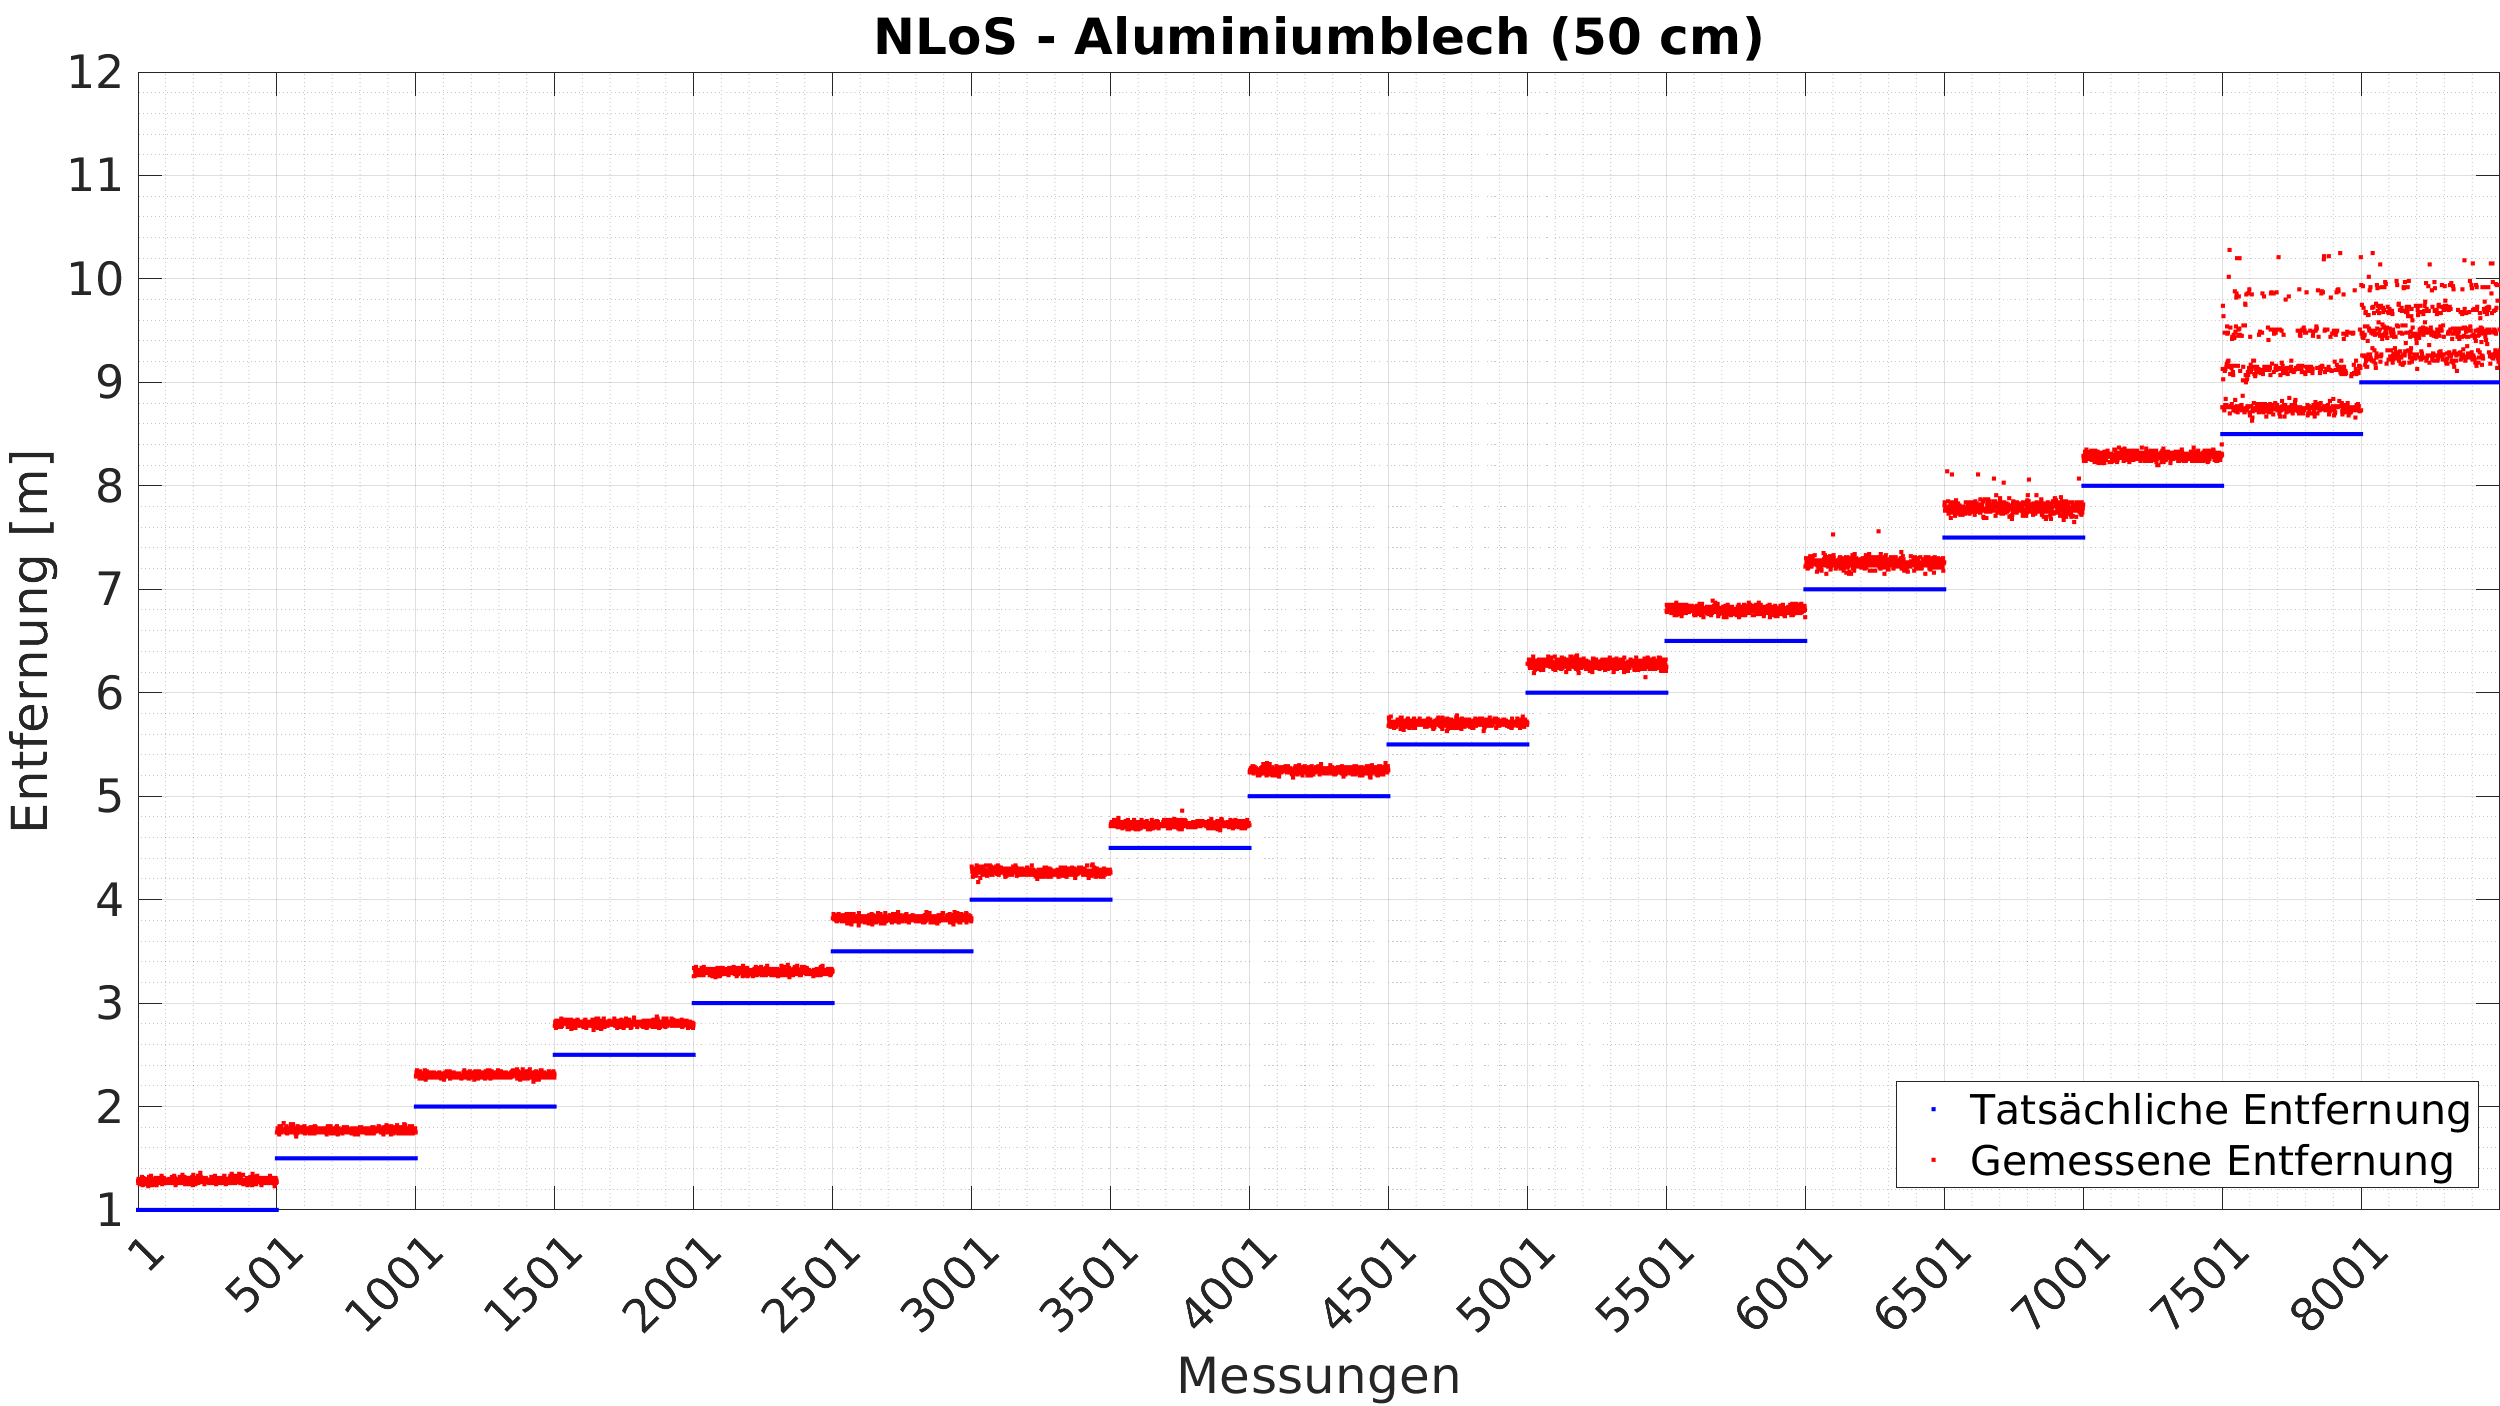
\includegraphics[scale=0.14]{entfernungsmessung_2018_01_20_nlos_metal}
		
		\column{0.5\linewidth}
			\centering
			
			NLOS mit Wasser
			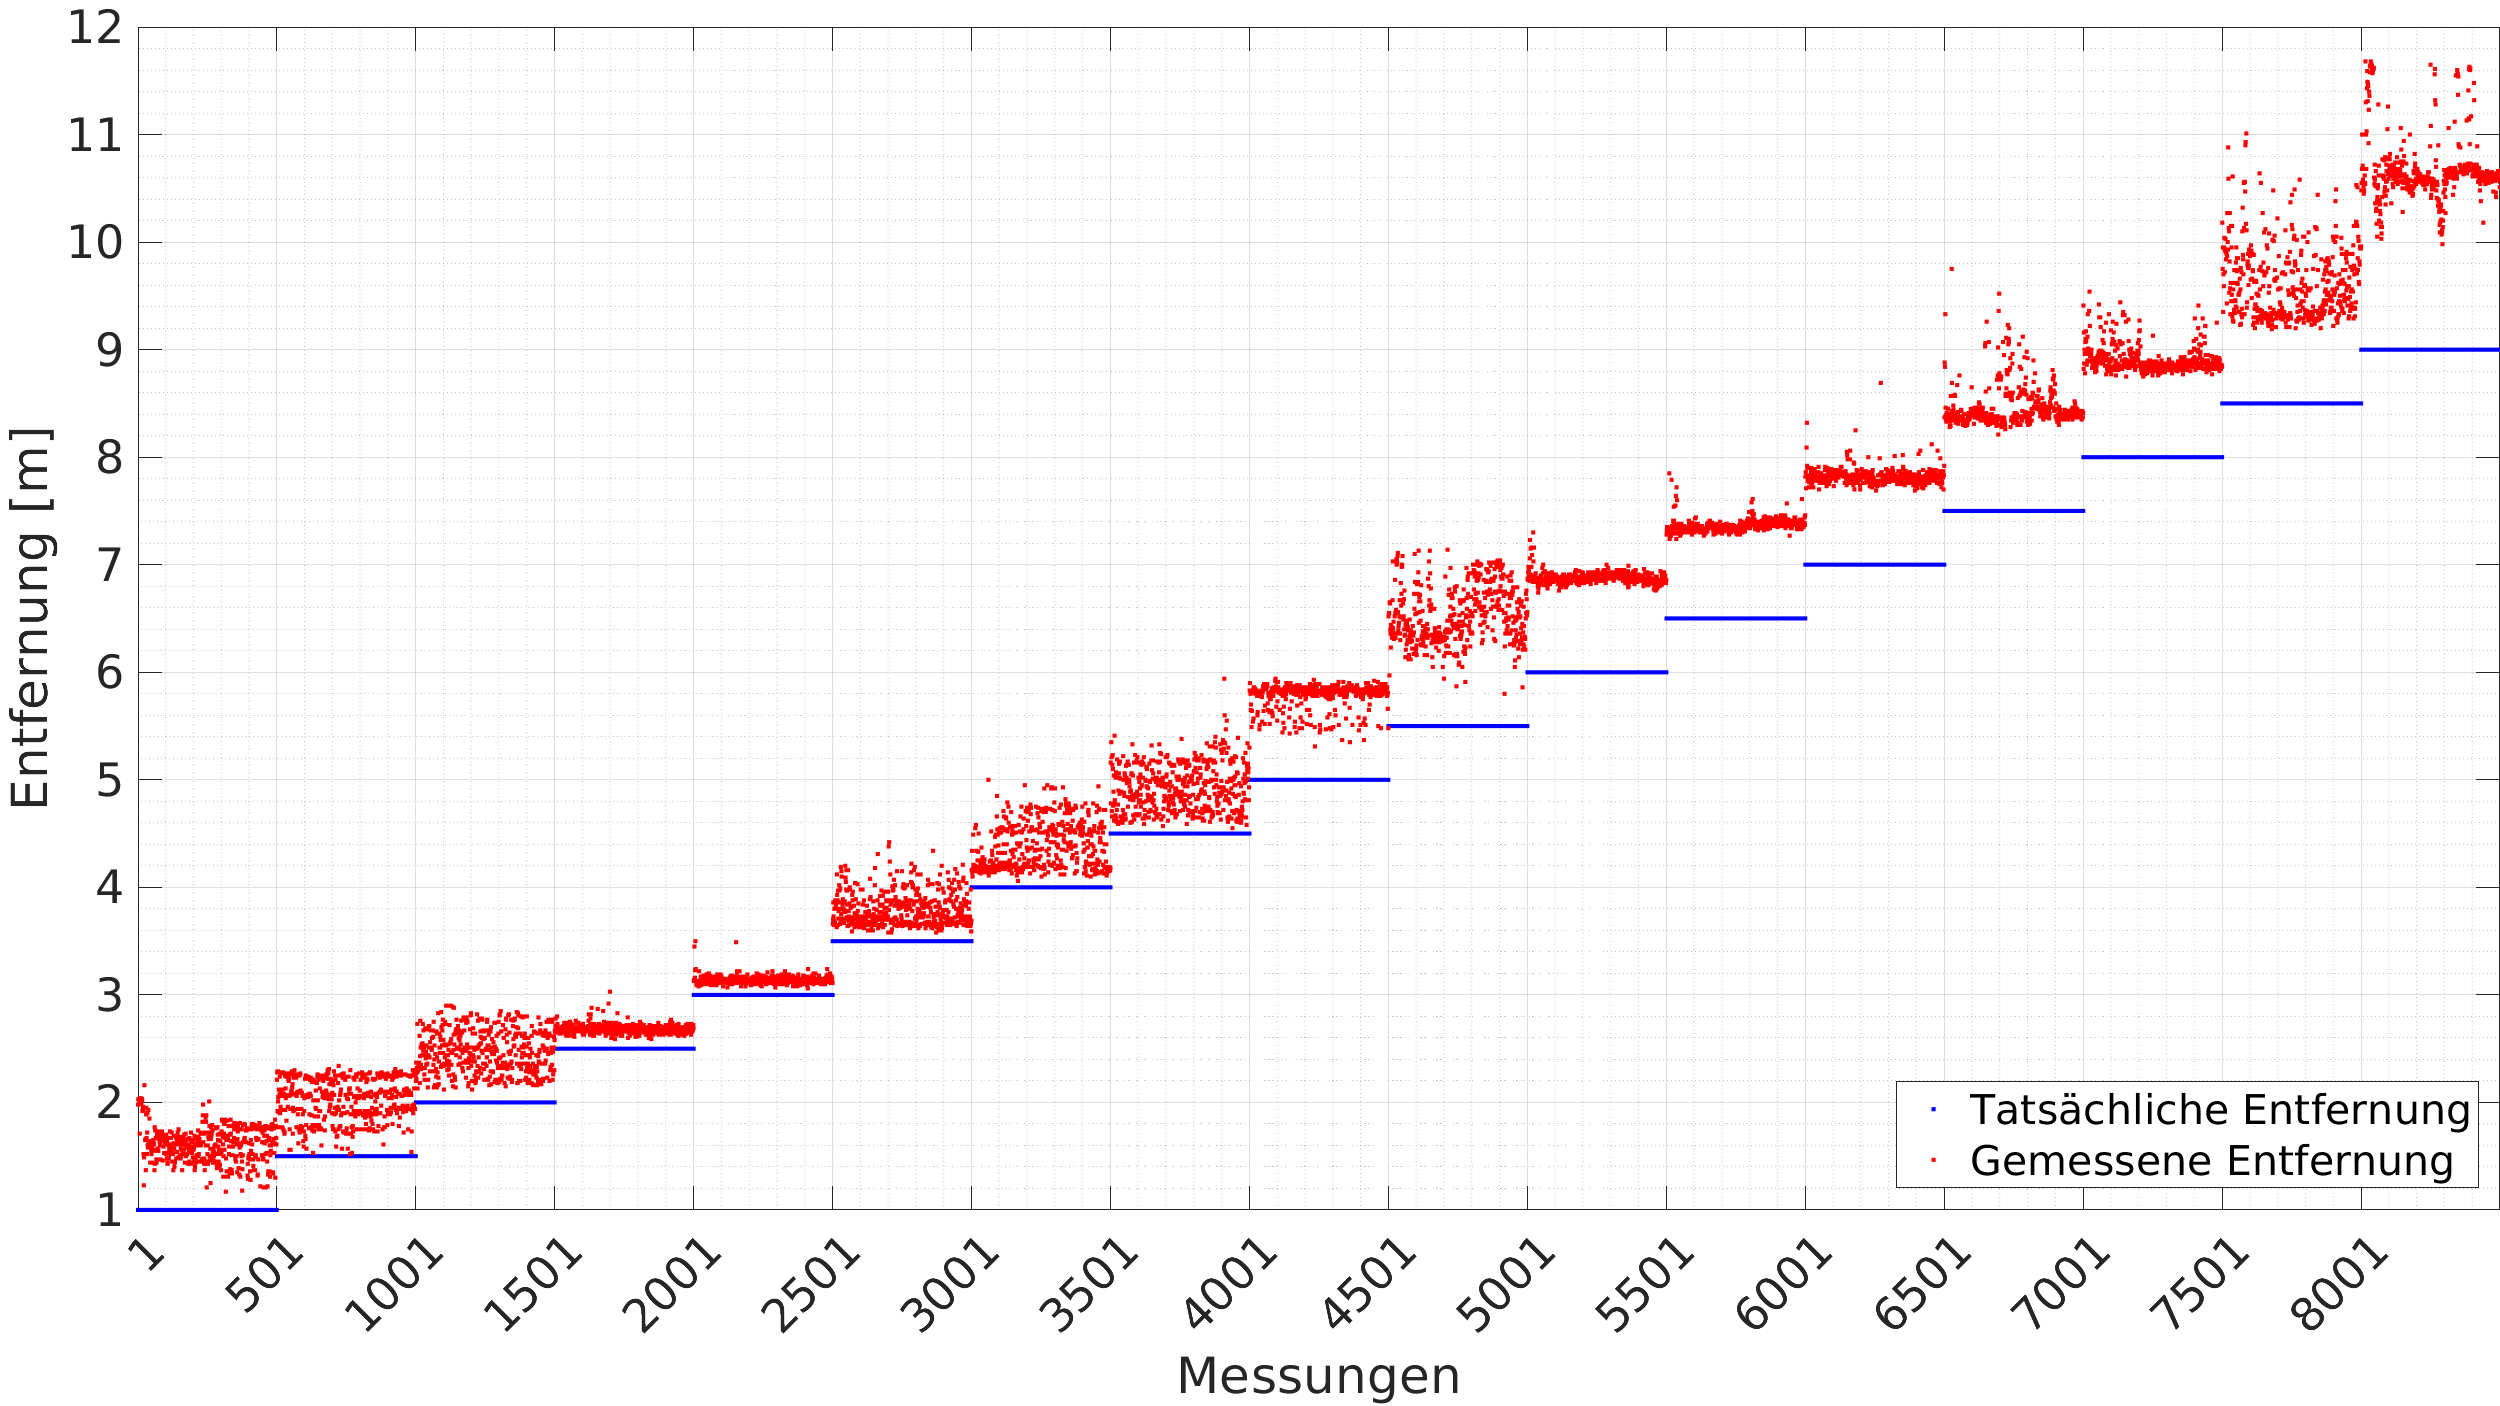
\includegraphics[scale=0.14]{entfernungsmessung_2018_01_20_nlos_water}
			
			NLOS mit Metall (2)
			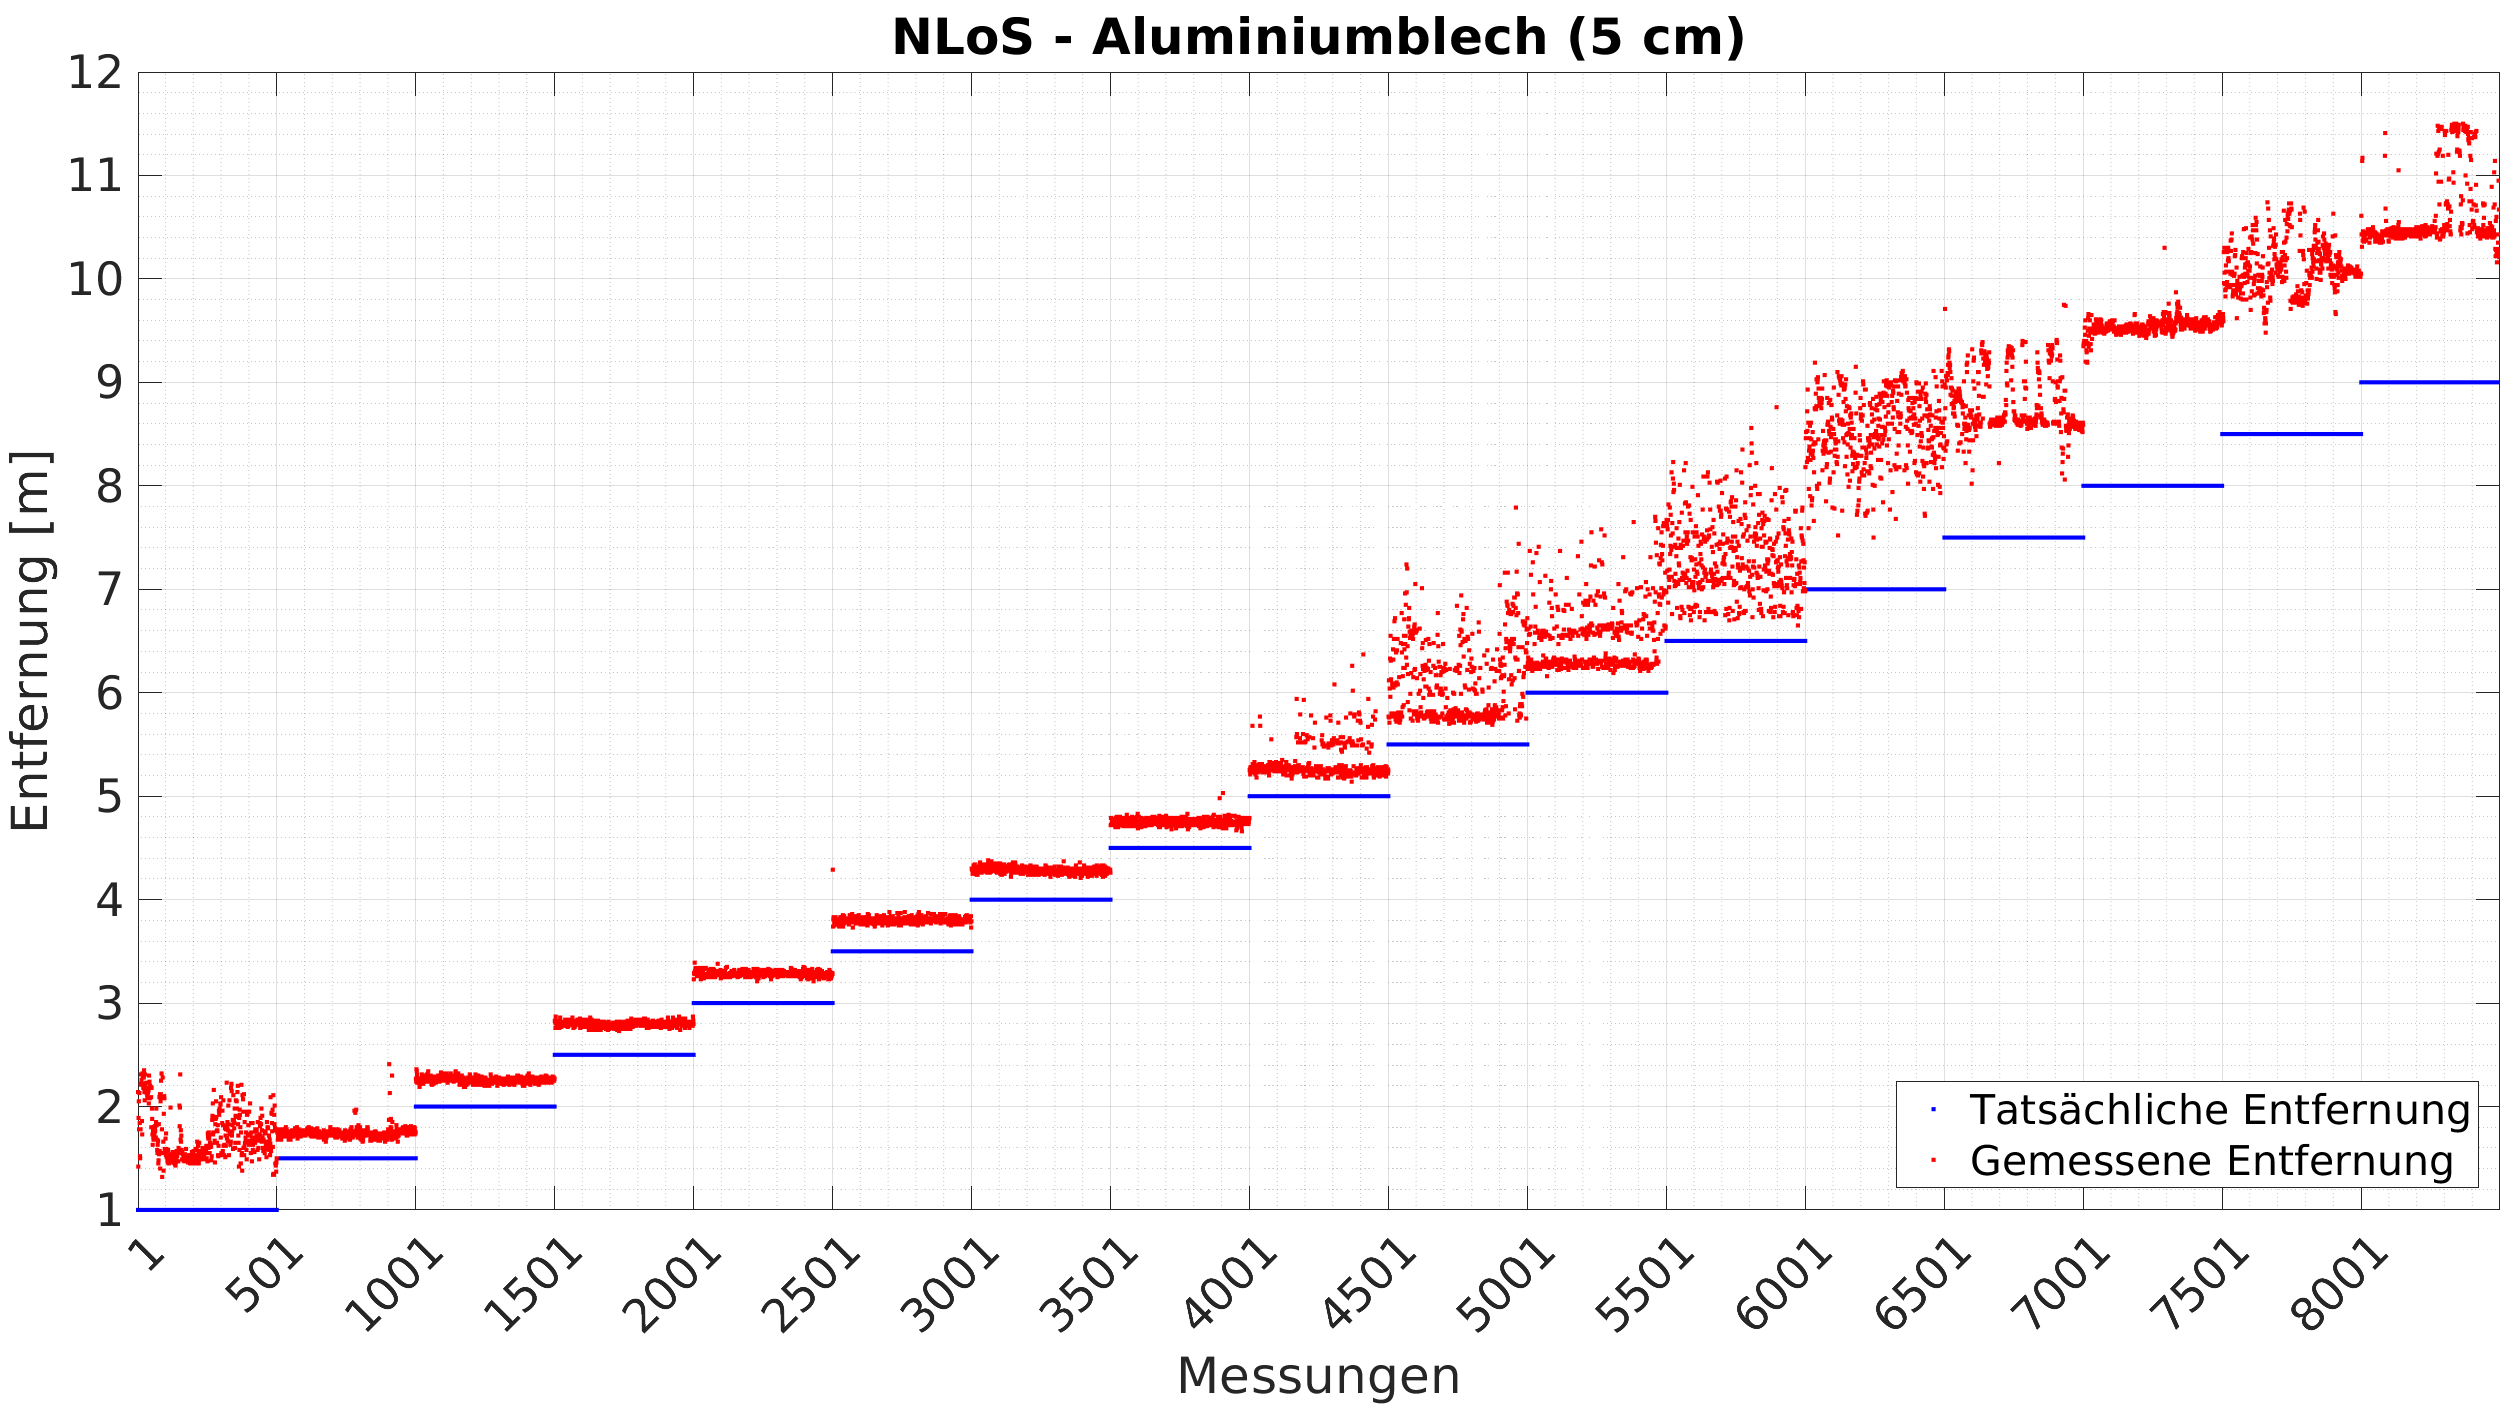
\includegraphics[scale=0.14]{entfernungsmessung_2018_01_20_nlos_metal2}
	\end{columns}
\end{frame}

%%%%%%%%%%%%%%%%%%%%%%%%%%%%%%%%%%%%%%%%%%%%%%%%%%%%%%%%%%%%%%%%%%%%%%%%%%%%%%%%
%
% 
%
%%%%%%%%%%
\begin{frame}
	\frametitle{Theorie 1/3: Gaussverteilung}
	\begin{columns}
		\column{0.5\linewidth}
			\centering
			2D
		
		\column{0.5\linewidth}
			\centering
			Multivariat
			%https://upload.wikimedia.org/wikipedia/commons/9/95/Multivariate_normal_sample.svg
	\end{columns}
\end{frame}


%%%%%%%%%%%%%%%%%%%%%%%%%%%%%%%%%%%%%%%%%%%%%%%%%%%%%%%%%%%%%%%%%%%%%%%%%%%%%%%%
%
%
%
%%%%%%%%%%
\begin{frame}
	\frametitle{Theorie 2/3: Monte Carlo mit Sum of Gaussian (SOG)}
	\begin{columns}
		\column{0.5\linewidth}
			\centering
			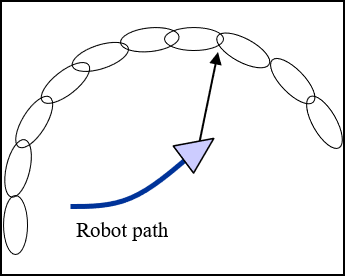
\includegraphics[scale=0.5]{blanco2008efficient_fig10a}		
		
		\column{0.5\linewidth}
			\centering
			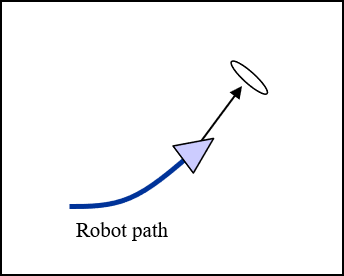
\includegraphics[scale=0.5]{blanco2008efficient_fig10b}
	\end{columns}
\end{frame}


%%%%%%%%%%%%%%%%%%%%%%%%%%%%%%%%%%%%%%%%%%%%%%%%%%%%%%%%%%%%%%%%%%%%%%%%%%%%%%%%
%
%
%
%%%%%%%%%%
\begin{frame}
	\frametitle{Theorie 3/3:  Monte Carlo mit Hilfs-Partikel-Filter}
	\begin{columns}
		\column{0.5\linewidth}
			\centering
			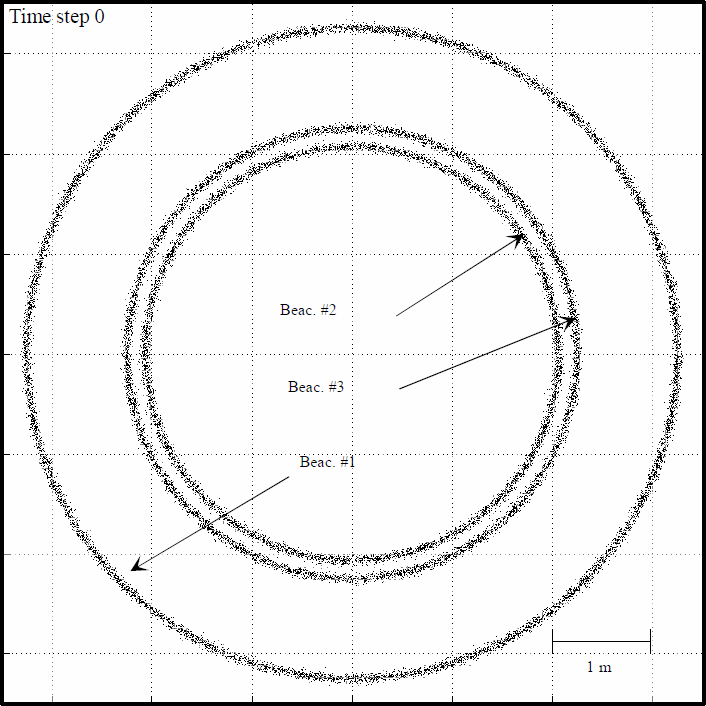
\includegraphics[scale=0.4]{blanco2008pure_fig3e}
		
		\column{0.5\linewidth}
			\centering			
			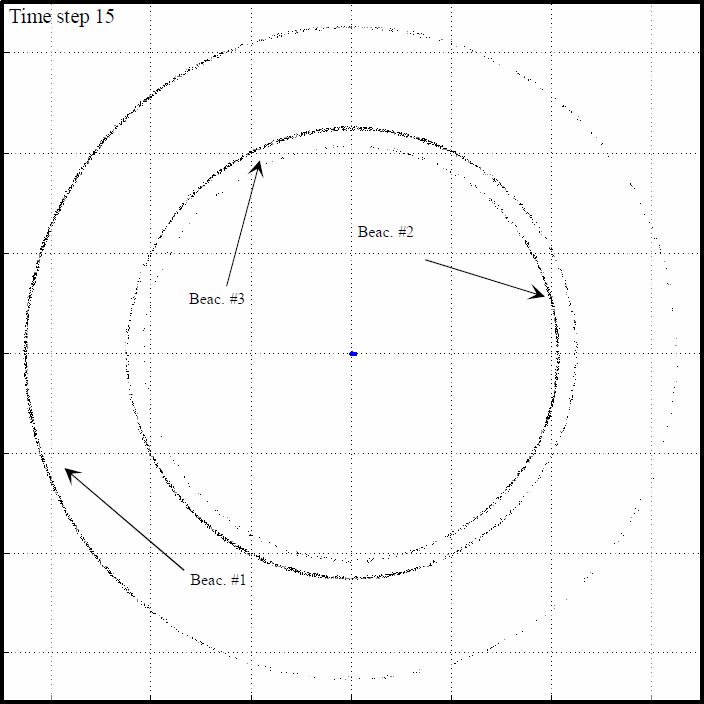
\includegraphics[scale=0.23]{blanco2008pure_fig3f}
			\par\bigskip
			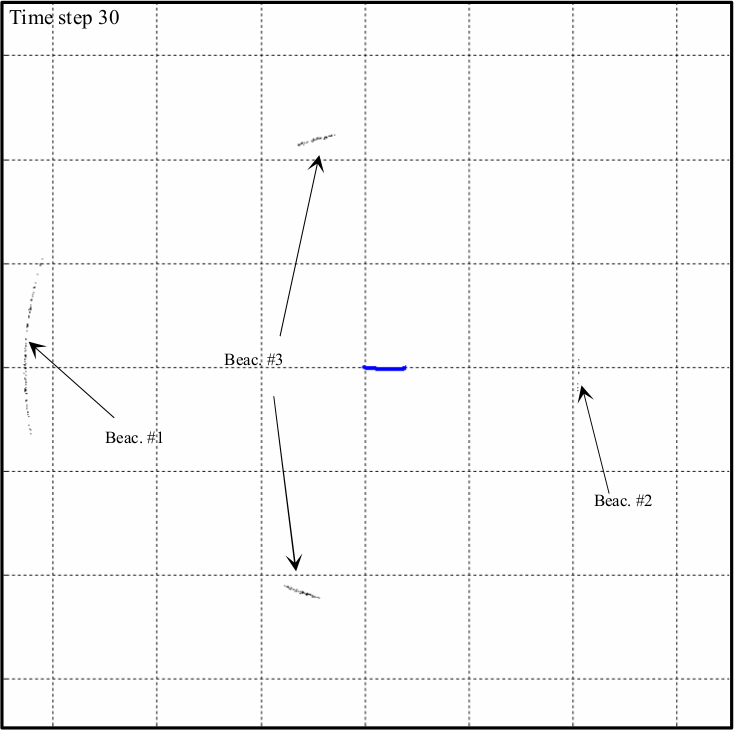
\includegraphics[scale=0.23]{blanco2008pure_fig3g}
	\end{columns}
\end{frame}


%%%%%%%%%%%%%%%%%%%%%%%%%%%%%%%%%%%%%%%%%%%%%%%%%%%%%%%%%%%%%%%%%%%%%%%%%%%%%%%%
%
% 
%
%%%%%%%%%%
\begin{frame}
	\frametitle{Fazit}
	\begin{itemize}
		\item ...
		\item ...
	\end{itemize}
\end{frame}

%%%%%%%%%%%%%%%%%%%%%%%%%%%%%%%%%%%%%%%%%%%%%%%%%%%%%%%%%%%%%%%%%%%%%%%%%%%%%%%%
%
% 
%
%%%%%%%%%%
%\begin{frame}
%\frametitle{Frame Template}
%This is a text in first frame. This is a text in first frame. This is a text in first frame.
%\end{frame}





\end{document}